\section{Empirical analysis of improvement}

In order to empirically assess the space efficiency of our improvement, we
measured the size of the interlink data structure in the case of interlink
\emph{lists}, the previously proposed format, and in the case of interlink
\emph{sets}, our newly proposed format. We performed our measurements on the
mainnet for both Bitcoin and Litecoin. Our results are illustrated in
Figure~\ref{fig.set-list-vector-comparison} and are similar for both of these
coins. The figures assume that both coins have been velvet forked from their
geneses blocks to include the particular interlink vector format. This is
indicative of the future performance of velvet forking each blockchain to add
the respective interlink vector format.

The new data structure format yields savings of approximately $83\%$ on average.
Based on the theoretical analysis of Section~\ref{sec.construction}, we expect
to see approximately an improvement of $50\%$ in this structure. The extra
$33\%$ is due to the explosion of difficulty in the mining power in both
cryptocurrencies. The increased difficulty causes a lower variable difficulty
target, meaning that the lowest portions of the superblock levels remain
unoccupied, but are still accounted for in the interlink vector list approach.

\begin{figure}
   \centering
   \subcaptionbox[]{%
      \centering
      Bitcoin
   }
   [
       0.80\textwidth
   ]
   {
       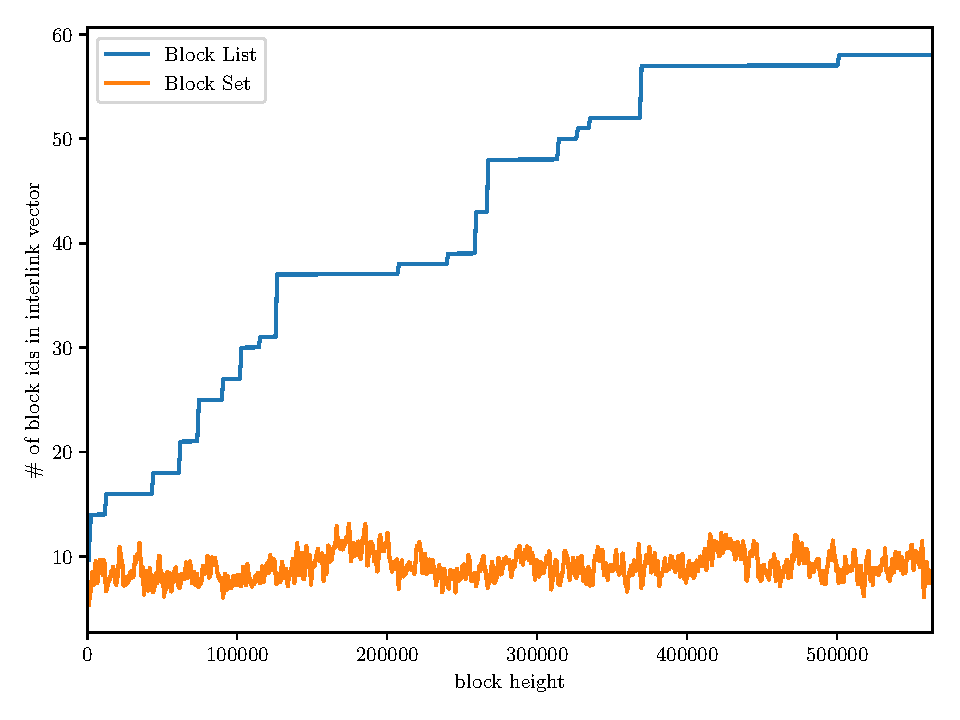
\includegraphics[width=0.85 \textwidth]
       {figures/interlink-vector-blocklist-vs-blockset.pdf}
   }
   \vskip 0pt
   \subcaptionbox[]{%
      \centering
      Litecoin
   }
   [
       0.80\textwidth
   ]
   {
       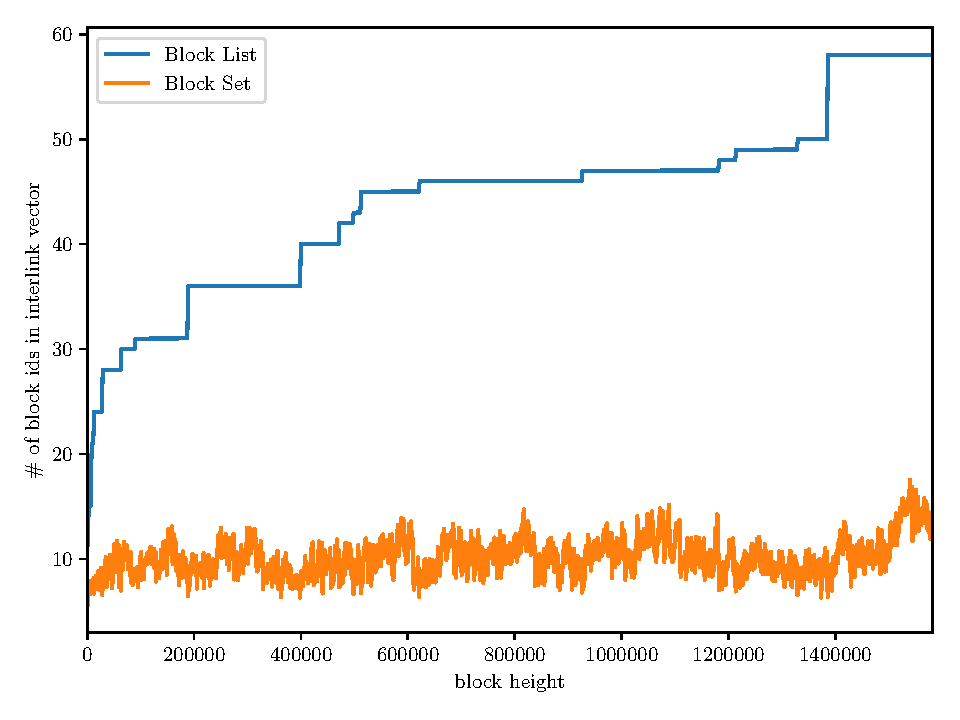
\includegraphics[width=0.85 \textwidth]
       {figures/interlink-vector-blocklist-vs-blockset-litecoin.pdf}
   }
   \caption{A comparison of interlink vector sizes for interlink block lists (previous work) and interlink block sets (this work) in two popular blockchains (lower is better)}
   \label{fig.set-list-vector-comparison}
\end{figure}

Based on the sizes attained in the interlink vector, we organized the interlink
vector into Merkle trees for both the list and the set structure and created
proofs-of-inclusion of which we measured the size. Our results are illustrated
in Figure~\ref{fig.set-list-proof-comparison}.

\begin{figure*}[h]
\begin{center}
  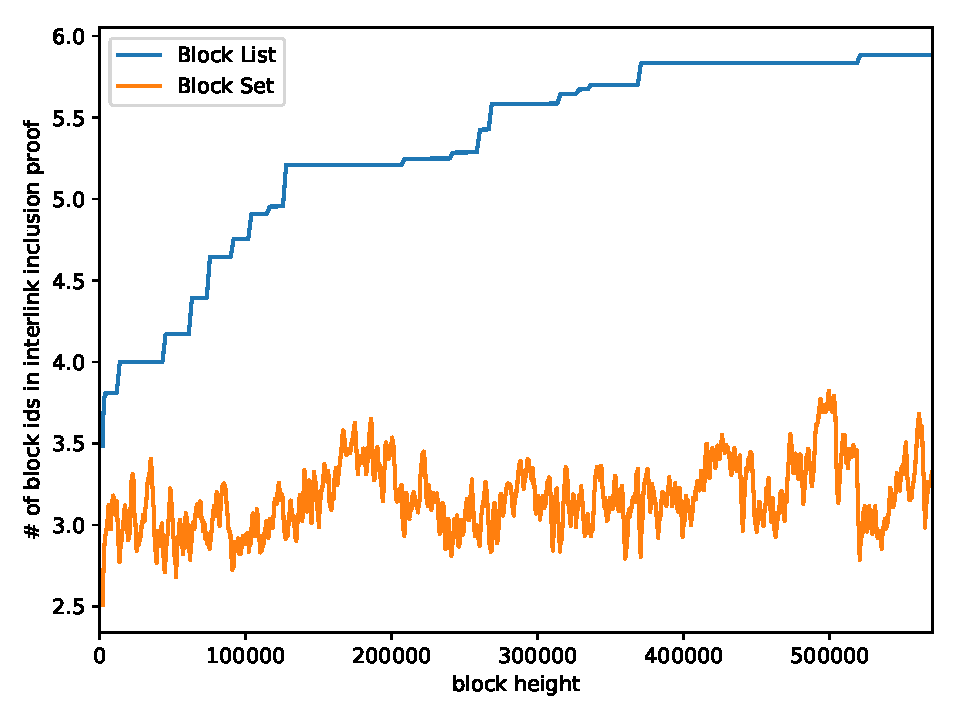
\includegraphics[width=0.95\textwidth]{figures/interlink-proof-list-vs-set.pdf}
  \caption{A comparison of a proof-of-inclusion size in the case of interlink block lists (previous work) and interlink block sets (this work) in Bitcoin (lower is better)}
  \label{fig.set-list-proof-comparison}
  \end{center}
\end{figure*}

\begin{figure*}[h]
\begin{center}
  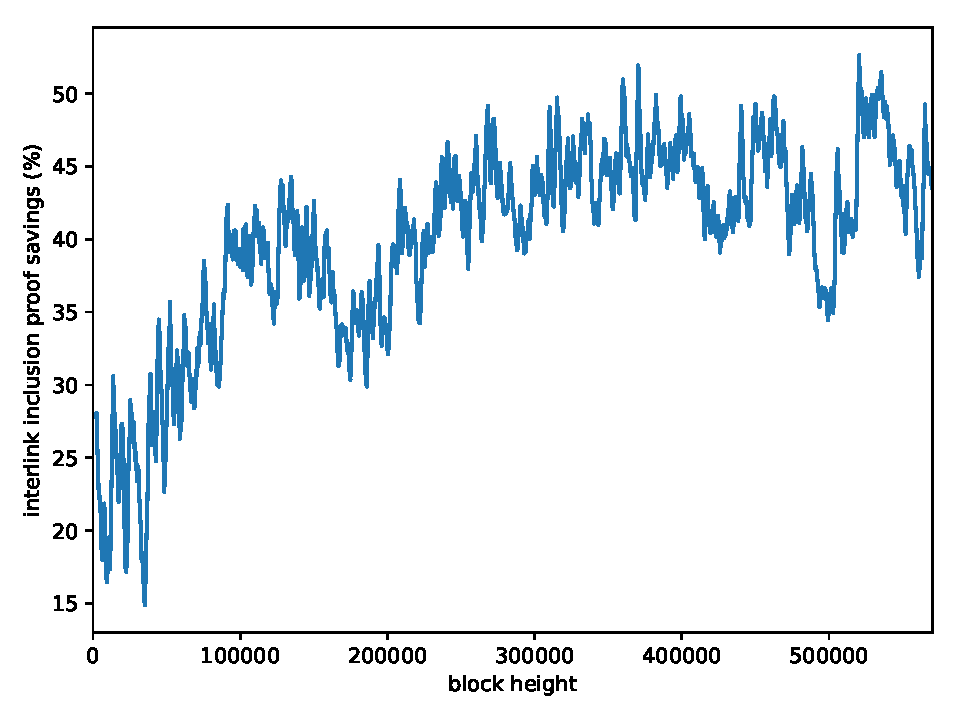
\includegraphics[width=0.95\textwidth]{figures/interlink-proof-savings-from-blockset.pdf}
  \caption{Percentile savings of our block set construction compared to the
           previously known block list construction.}
  \label{fig.set-list-proof-comparison}
  \end{center}
\end{figure*}

\TODO{TODO: Explain Figure~\ref{fig.set-list-proof-comparison}}

\begin{table}[h!]
  \begin{center}
    \begin{tabular}{|c|cc|cc|cc|}
      \hline
      & \multicolumn{2}{c|}{\bf Interlink size}
      & \multicolumn{2}{c|}{\bf Proof-of-inclusion size}
      & \multicolumn{2}{c|}{\bf NIPoPoW size}\\
      & blockids & bytes & hashes & bytes & KB\\
      \hhline{-------}
      \textbf{Interlink lists}&
      5 & 7 & 35 & 25 & 44.79\\
      \hline
      \makecell{\bf Interlink sets\\(this work)}&
      5 & 7 & 35 & 25 & 28.28\\
      \hline
    \end{tabular}
    \vspace{10pt}
    \caption{A comparison of the two interlink constructions in terms of size.}
    \label{tab.savings}
  \end{center}
\end{table}

We summarize the savings of our construction in Table~\ref{tab.savings}. The
table was constructed by inspecting the current version of the Bitcoin
blockchain at the time of writing. The interlink size column shows the average
interlink vector size, in the number of blockids and in concrete bytes assuming
the \texttt{SHA256} function is used (as in Bitcoin). The proof-of-inclusion
size column shows the average size of a Merkle proof-of-inclusion, in the number
of hashes and in bytes, when the interlink vector is compacted into a Merkle
tree using \texttt{SHA256} (as in Bitcoin). Finally, the NIPoPoW size column
shows the size of a NIPoPoW in kilobytes. The NIPoPoW sizes are calculated
assuming Bitcoin had included the respective interlink Merkle tree root in their
headers since genesis. We measured the size of suffix-proof NIPoPoWs based on
the recommended parameter $m = 15$~\cite{nipopows} assuming a chain size of $|C|
= 563{,}451$. The number of blocks in a NIPoPoW is $(m(log |C| − log m) + 1.5m)
= 250$ in expectation. For the final size calculation of the NIPoPoW, we
included all the data required, including the proofs-of-inclusion as well as the
auxiliary block header data needed. Our results indicate $79\%$ savings in the
interlink sizes and $37\%$ savings in the NIPoPoW sizes.
